\documentclass[12pt]{article}

% ---- Core packages ----
\usepackage[margin=1in]{geometry}
\usepackage{setspace}
\usepackage{xcolor}
\usepackage{graphicx}
\usepackage{titlesec}
\usepackage{fontspec}      % XeLaTeX/LuaLaTeX
\usepackage{fancyhdr}
\usepackage{enumitem}
\usepackage{amsmath}
\usepackage[section]{placeins} 
\usepackage[strings]{underscore} % make _ safe in text and in arguments like \cite{...}
\usepackage{hyperref}             % load before biblatex
\usepackage{booktabs}

% ---- Bibliography: biblatex (modern, no natbib) ----
\usepackage[backend=biber,style=authoryear]{biblatex}
\addbibresource{references.bib}

% ---- Fonts (Overleaf has Roboto & Carlito) ----
\defaultfontfeatures{Ligatures=TeX}
\IfFontExistsTF{Roboto}{%
  \setmainfont{Roboto}%
}{%
  \setmainfont{Latin Modern Roman}%
}
\IfFontExistsTF{Roboto}{%
  \newfontfamily\robotosans{Roboto}[Scale=MatchLowercase]%
}{%
  \newfontfamily\robotosans{Latin Modern Sans}[Scale=MatchLowercase]%
}
\IfFontExistsTF{Carlito}{%
  \newfontfamily\carlito{Carlito}[Scale=MatchLowercase]%
}{%
  \newfontfamily\carlito{Latin Modern Sans}[Scale=MatchLowercase]%
}
% convenient alias
\newcommand{\roboto}{\robotosans}

% ---- Colors & section titles ----
\definecolor{projectblue}{HTML}{005F86}
\titleformat{\section}{\normalfont\color{projectblue}\bfseries\fontsize{22}{30}\selectfont}{\thesection.}{0.5em}{}
\titleformat{\subsection}{\normalfont\color{projectblue}\bfseries\fontsize{16}{22}\selectfont}{\thesubsection}{0.5em}{}
\titleformat{\subsubsection}{\normalfont\color{projectblue}\bfseries\fontsize{12}{16}\selectfont}{\thesubsubsection}{0.5em}{}

% ---- Lists ----
\setlist[itemize]{leftmargin=1.2em}
\setlist[enumerate]{leftmargin=1.5em}

% ---- Bibliography heading ----
\defbibheading{references}{%
  {\normalfont\color{projectblue}\bfseries\fontsize{16}{22}\selectfont #1\par}
}

% ---- Inline code: safe for _, %, \, etc. ----
\newcommand{\inlinecode}[1]{\texttt{\detokenize{#1}}}

% ---- Header / footer ----
\setlength{\headheight}{32pt}
\pagestyle{fancy}
\fancyhf{}
\fancyhead[L]{%
    {\roboto\textbf{GROUP WORK PROJECT \# }1}\\
    {\roboto\textbf{Group Number: }11231}%
}
\fancyhead[R]{%
    {\carlito MScFE 600: FINANCIAL DATA}\\
}
\fancyfoot[C]{\thepage}

\begin{document}

\setcounter{section}{1}
\section{Yield Curve Modeling}

\bigskip

\subsection{Data Acquisition}
\begin{spacing}{1.15}
This section documents how the German government zero-coupon curve was sourced and validated as the foundation for the Nelson--Siegel and Cubic-Spline modeling tasks.

\subsubsection{Data Source and Coverage}
\begin{itemize}
    \item \textbf{Provider:} Deutsche Bundesbank SDMX REST API \parencite{bundesbank_rest_api}\\(dataset \inlinecode{D.I.ZST.ZI.EUR.S1311.B.A604}  \parencite{bundesbank_zero_coupon}.
    \item \textbf{Instrument set:} Zero-coupon yield curve for central government debt denominated in EUR.
    \item \textbf{Tenor breadth:} Residual maturities from 0.5 years (\inlinecode{R005X}) through 30 years (\inlinecode{R30XX}), covering each annual bucket in between. This satisfies the assignment requirement to span short- through long-term maturities (see the \emph{Description} section of \cite{bundesbank_zero_coupon}).
\end{itemize}

\subsubsection{Why the Bundesbank Term-Structure Series Dataset}
\begin{itemize}
  \item \textbf{Alignment with assignment scope:} The coursework requires a government-securities yield curve. Within the Bundesbank dataset catalog \parencite{bundesbank_data_yields}, the ``Term structure of interest rates in the debt securities market---estimated values'' \cite{bundesbank_zero_coupon} is the only branch that delivers a full maturity ladder for \emph{federal - government} securities.
  \item \textbf{Daily frequency and audit trail:} The ``Listed Federal securities'' subcategory exposes daily values for each maturity, letting us capture the most recent business day and preserve a reproducible cache.
  \item \textbf{Ready-to-use zero-coupon points:} The published Nelson--Siegel--Svensson estimates provide desmoothed spot rates at residual maturities from 0.5 to 30 years. Using these points avoids manual bond stripping while giving a clean target for the Nelson--Siegel and Cubic-Spline models that we must implement.
  \item \textbf{Alternative categories ruled out:} Money-market and deposit-rate tables do not cover government bonds; per-ISIN price tables require custom stripping; The Pfandbriefe pertain to covered bonds, not sovereign issuance. The \emph{Description} section in \cite{bundesbank_zero_coupon} confirms that the SDMX key \inlinecode{D.I.ZST.ZI.EUR.S1311.B.A604} targets the desired government curve.
\end{itemize}

\subsubsection{Retrieval Workflow}
\begin{enumerate}
    \item Determine the candidate business date in the \inlinecode{Europe/Berlin} timezone. If the current calendar day is a weekend or German public holiday, walk back to the previous business day using the official holiday calendar (\inlinecode{holidays.Germany}).
    \item For each maturity code in the published Bundesbank metadata, construct the full key of the SDMX series for each residual maturity and request the corresponding CSV slice for the target date, instead of fetching the whole dataset \parencite{bundesbank_zero_coupon_download}.
    \item Parse the returned CSV, drop metadata rows, and coerce the values to floats. If any tenor is missing or marked ``No value available'', record the gap and continue checking.
    \item Abort the fetch if any maturities are absent after iterating the full set. This guardrail prevents partially populated curves from contaminating downstream modelling.
\end{enumerate}

\subsubsection{Quality Controls and Audit Trail}
\begin{itemize}
    \item \textbf{Completeness checks:} The script raises an explicit error listing the missing maturities; the lookback window can be extended temporarily if necessary.
    \item \textbf{Caching:} Each successful run writes a timestamped snapshot to \inlinecode{data/raw/}, embedding both the curve date and the fetch timestamp to support reproduction and regulatory audit needs.
    \item \textbf{Reproducibility:} The notebook cell fetches data deterministically and without random sampling or manual intervention, ensuring that the fitted models can be regenerated on demand.
\end{itemize}

\end{spacing}

\subsection{Exploratory Analysis}
\begin{spacing}{1.15}
Figure~\ref{fig:raw-curve} shows the Bundesbank zero-coupon curve for 9 October 2025, exhibiting a gently upward-sloping structure that flattens beyond the 20-year point. Short-term yields remain below 2\%, while the long end stabilises around 3.3\%. It provides a clean baseline for parametric and non-parametric fits.
\end{spacing}

\begin{figure}[htbp]
  \centering
  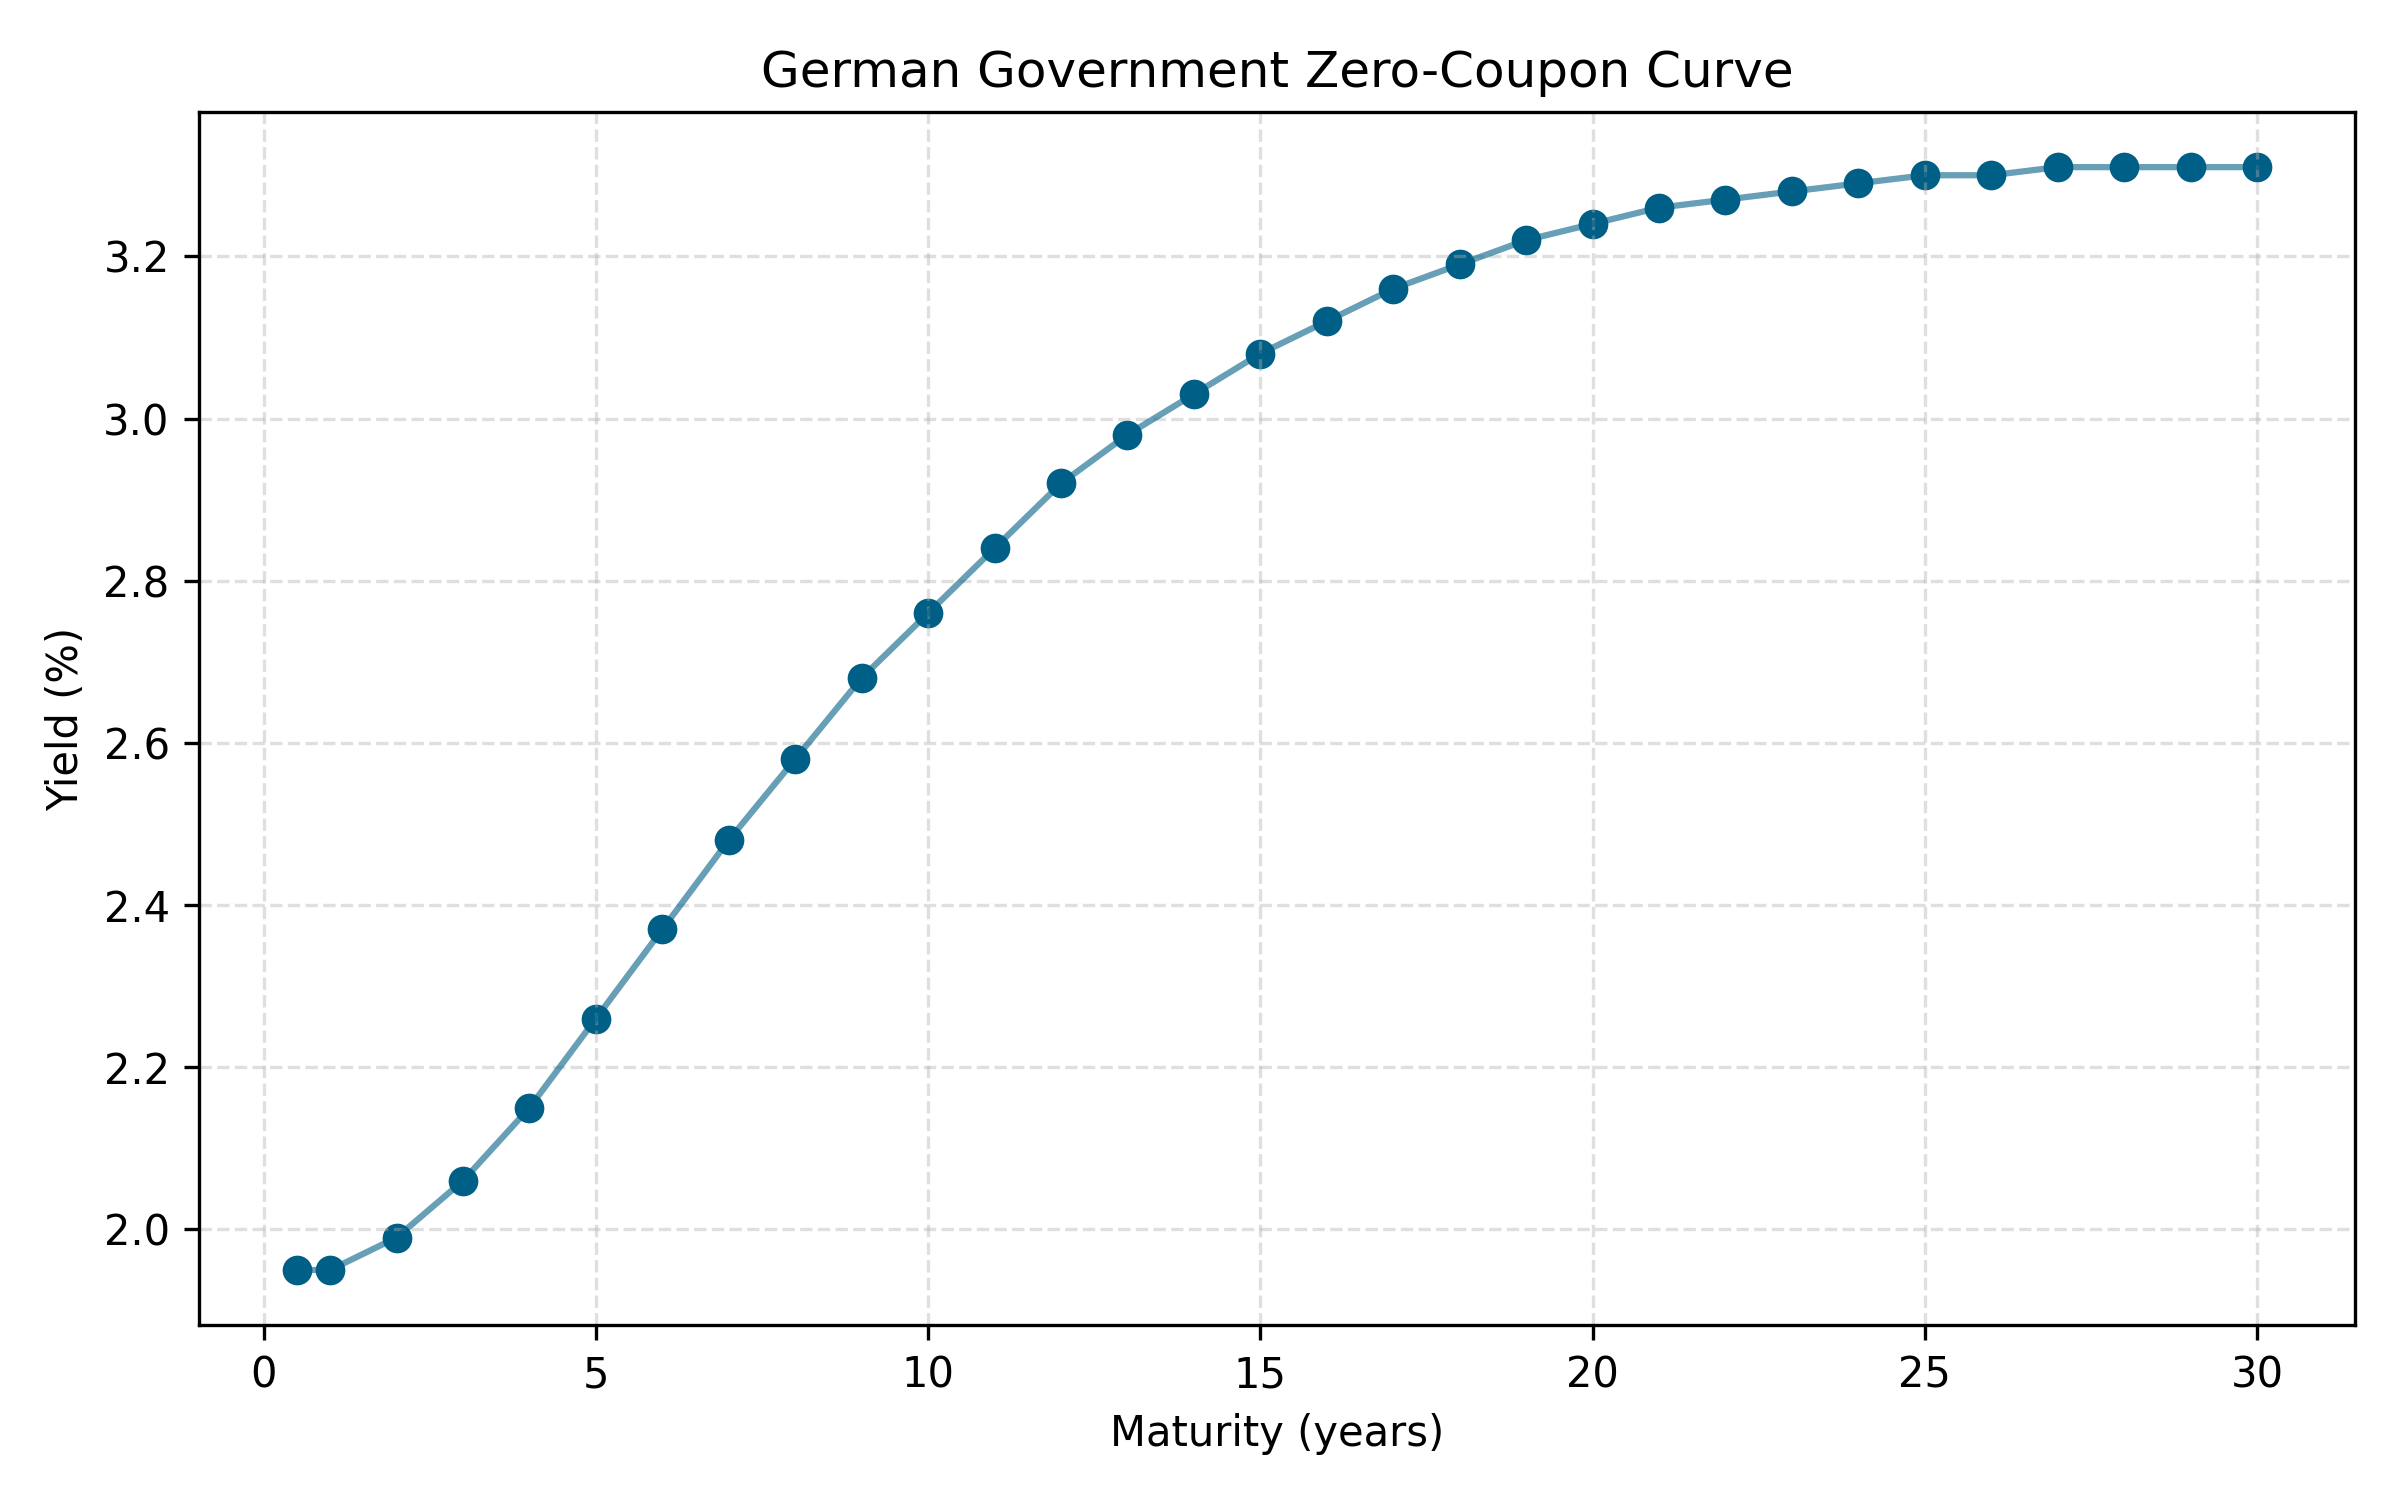
\includegraphics[width=0.8\textwidth]{../data/output/figure_raw_curve.png}
  \caption{Bundesbank zero-coupon yields by residual maturity on 9~October~2025. Source: \parencite{bundesbank_zero_coupon}.}
  \label{fig:raw-curve}
\end{figure}


\subsection{Nelson--Siegel Model}
\begin{spacing}{1.15}
We calibrate the four-parameter Nelson--Siegel (NS) specification \parencite{nelson_siegel_1987}, in which the spot rate at maturity $\tau$ is
\begin{equation}
  y_{\text{NS}}(\tau) = \beta_0 + \beta_1 \frac{1 - e^{-\tau/\tau_1}}{\tau/\tau_1} + \beta_2 \left( \frac{1 - e^{-\tau/\tau_1}}{\tau/\tau_1} - e^{-\tau/\tau_1} \right).
\end{equation}
The factors $(\beta_0, \beta_1, \beta_2)$ capture the level, slope, and medium-term curvature respectively, while $\tau_1$ controls the decay of the exponential loading. Parameters are estimated with non-linear least squares against the 0.5--30 year cross-section. The fitted curve (Figure~\ref{fig:ns-fit}) follows the broad shape of the data but leaves residual structure at both extremes, signalling the need for additional flexibility.

Table~\ref{tab:param-summary} reports the calibrated coefficients. The level factor $\beta_0$ settles near 3.68\%, consistent with long-dated yields, whereas the negative slope factor reflects the downward tilt between the short and long ends observed in the data.
\end{spacing}

\begin{figure}[htbp]
  \centering
  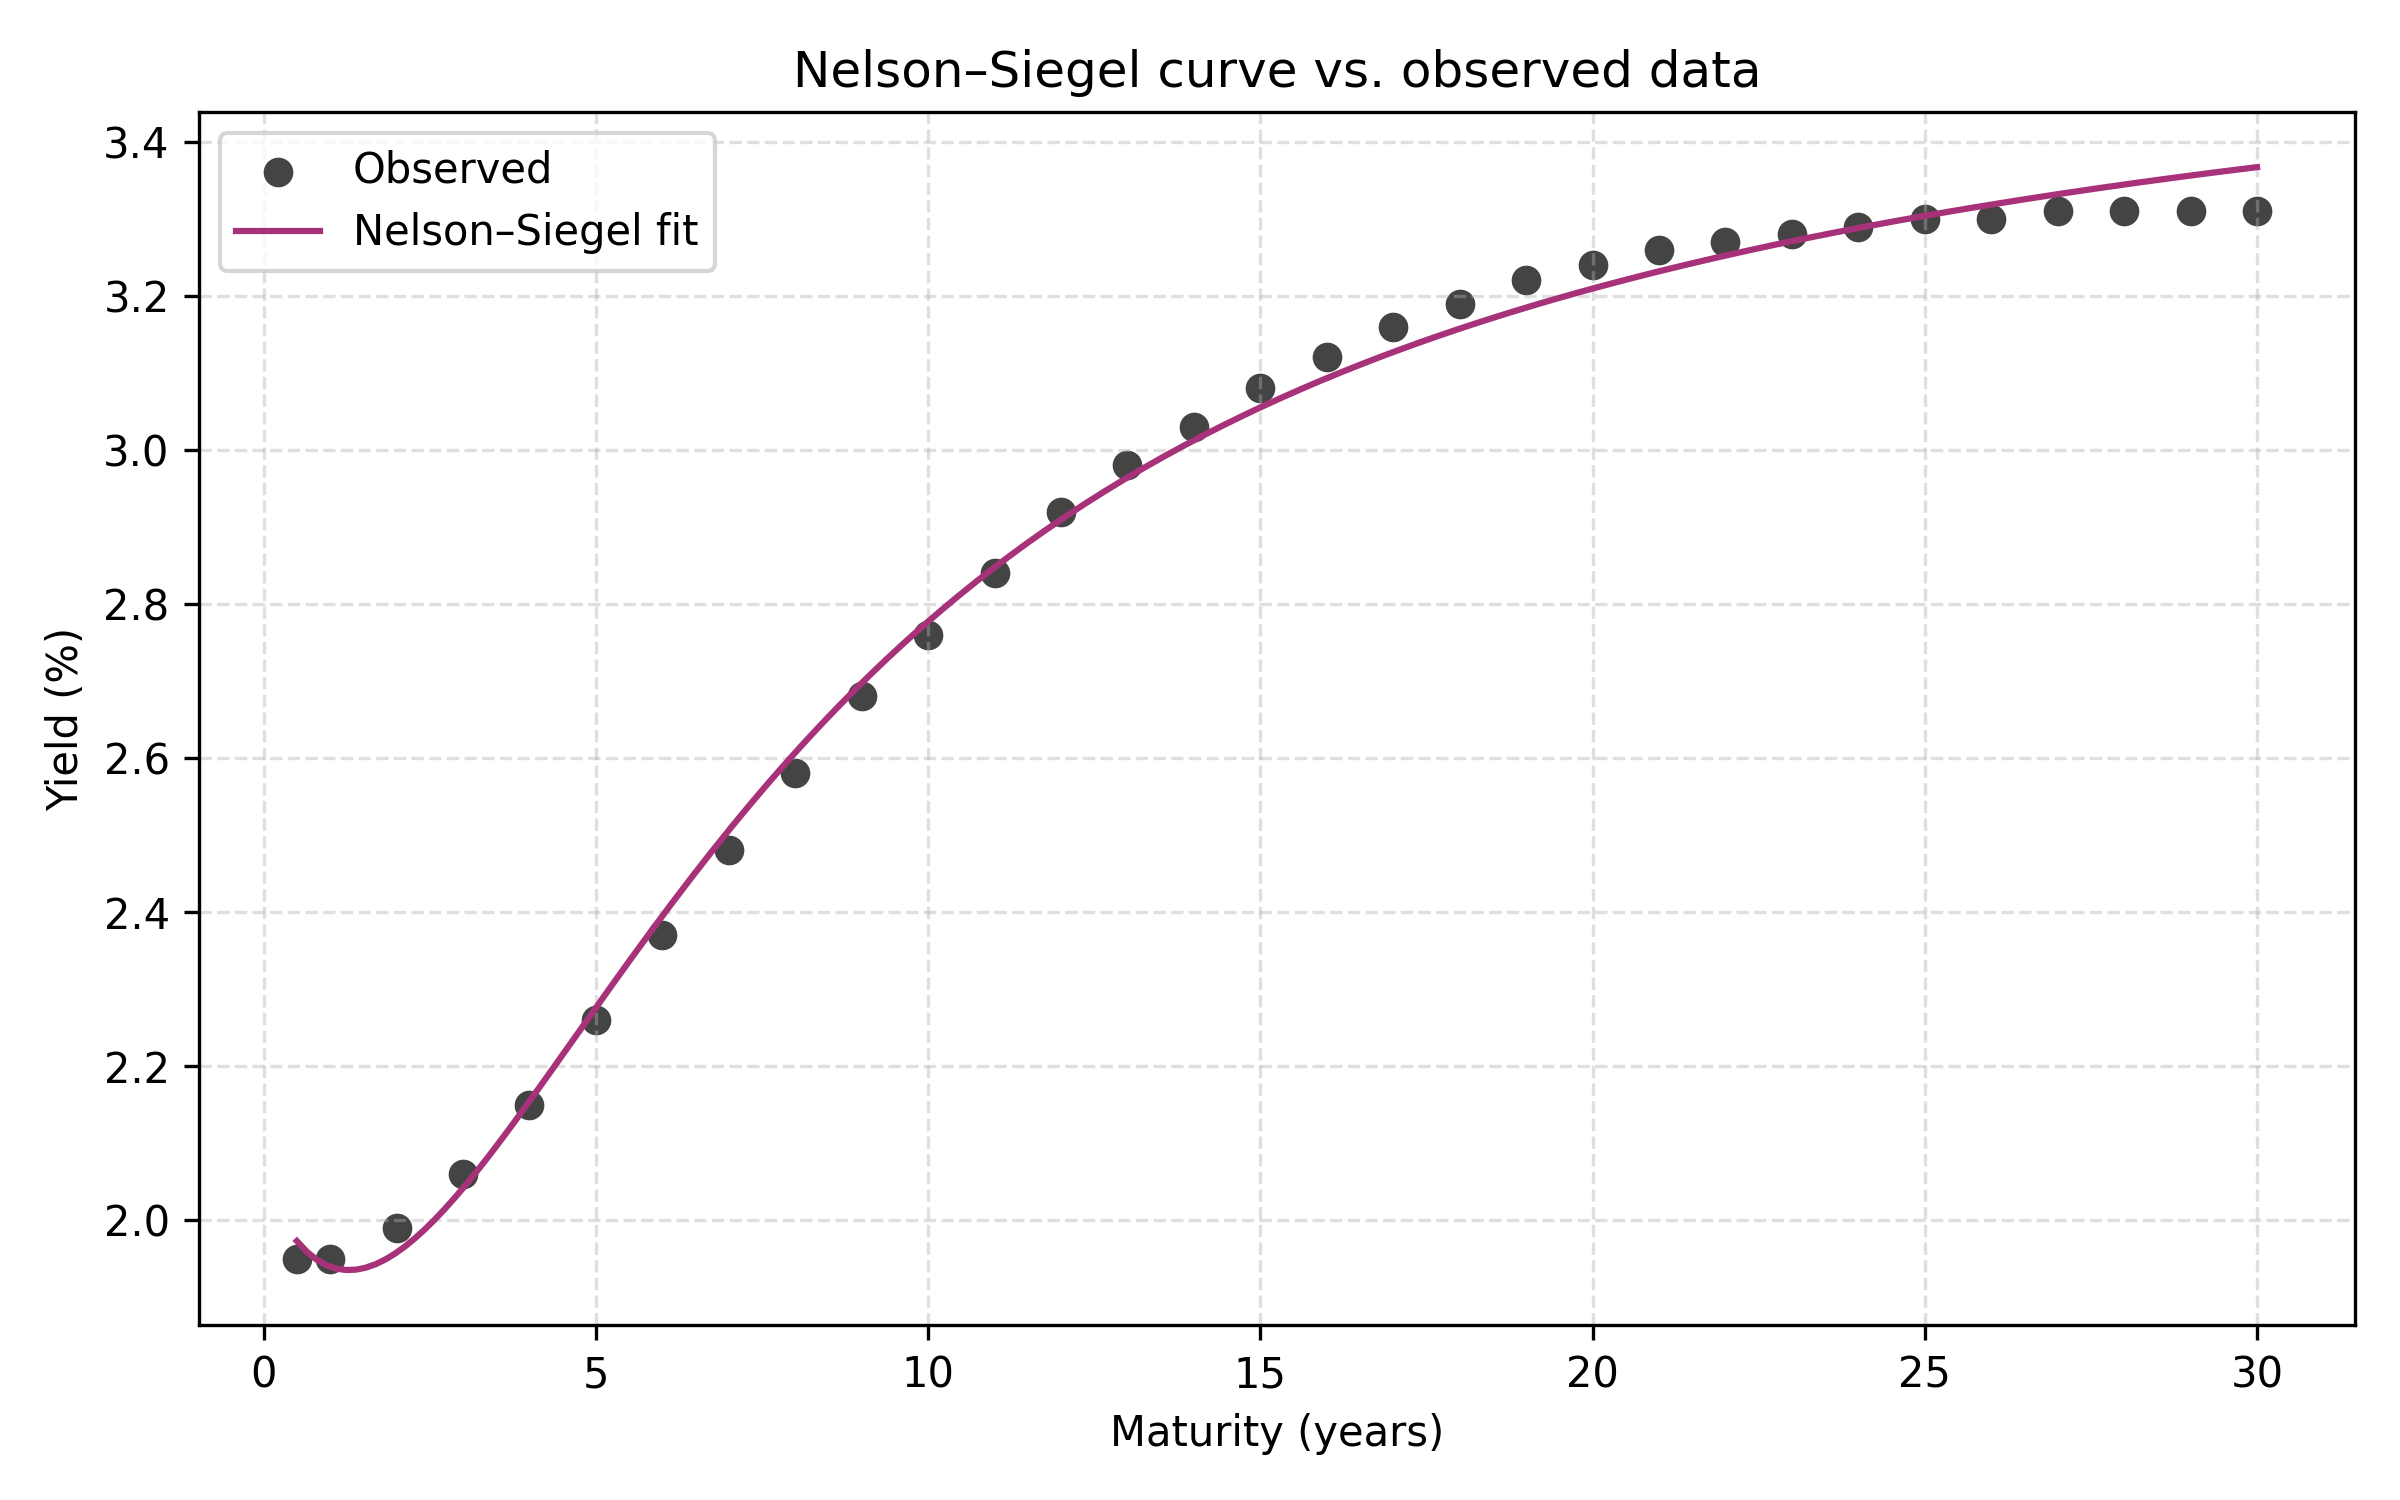
\includegraphics[width=0.8\textwidth]{../data/output/figure_ns_fit.png}
  \caption{Nelson--Siegel fit versus observed yields.}
  \label{fig:ns-fit}
\end{figure}

\FloatBarrier
\subsection{Nelson--Siegel--Svensson Extension}
\begin{spacing}{1.15}
To capture long-end curvature we extend the model with the Nelson--Siegel--Svensson (NSS) term \parencite{diebold_li_2006, ecb_yield_curve_2018}. The NSS curve augments the NS structure with an additional exponential hump:
\begin{equation}
  y_{\text{NSS}}(\tau) = y_{\text{NS}}(\tau) + \beta_3 \left( \frac{1 - e^{-\tau/\tau_2}}{\tau/\tau_2} - e^{-\tau/\tau_2} \right),
\end{equation}
introducing parameters $(\beta_3, \tau_2)$ that target long-term dynamics. Figure~\ref{fig:nss-fit} illustrates the near-perfect alignment between NSS estimates and observed yields; the additional curvature term corrects the slight under- and over-shoots left by the NS curve. Parameter values in Table~\ref{tab:param-summary} show how $\beta_3$ adds a second hump around eight years, while $\tau_1$ shifts upward to focus the original curvature on the mid-belly.
\end{spacing}

\begin{figure}[htbp]
  \centering
  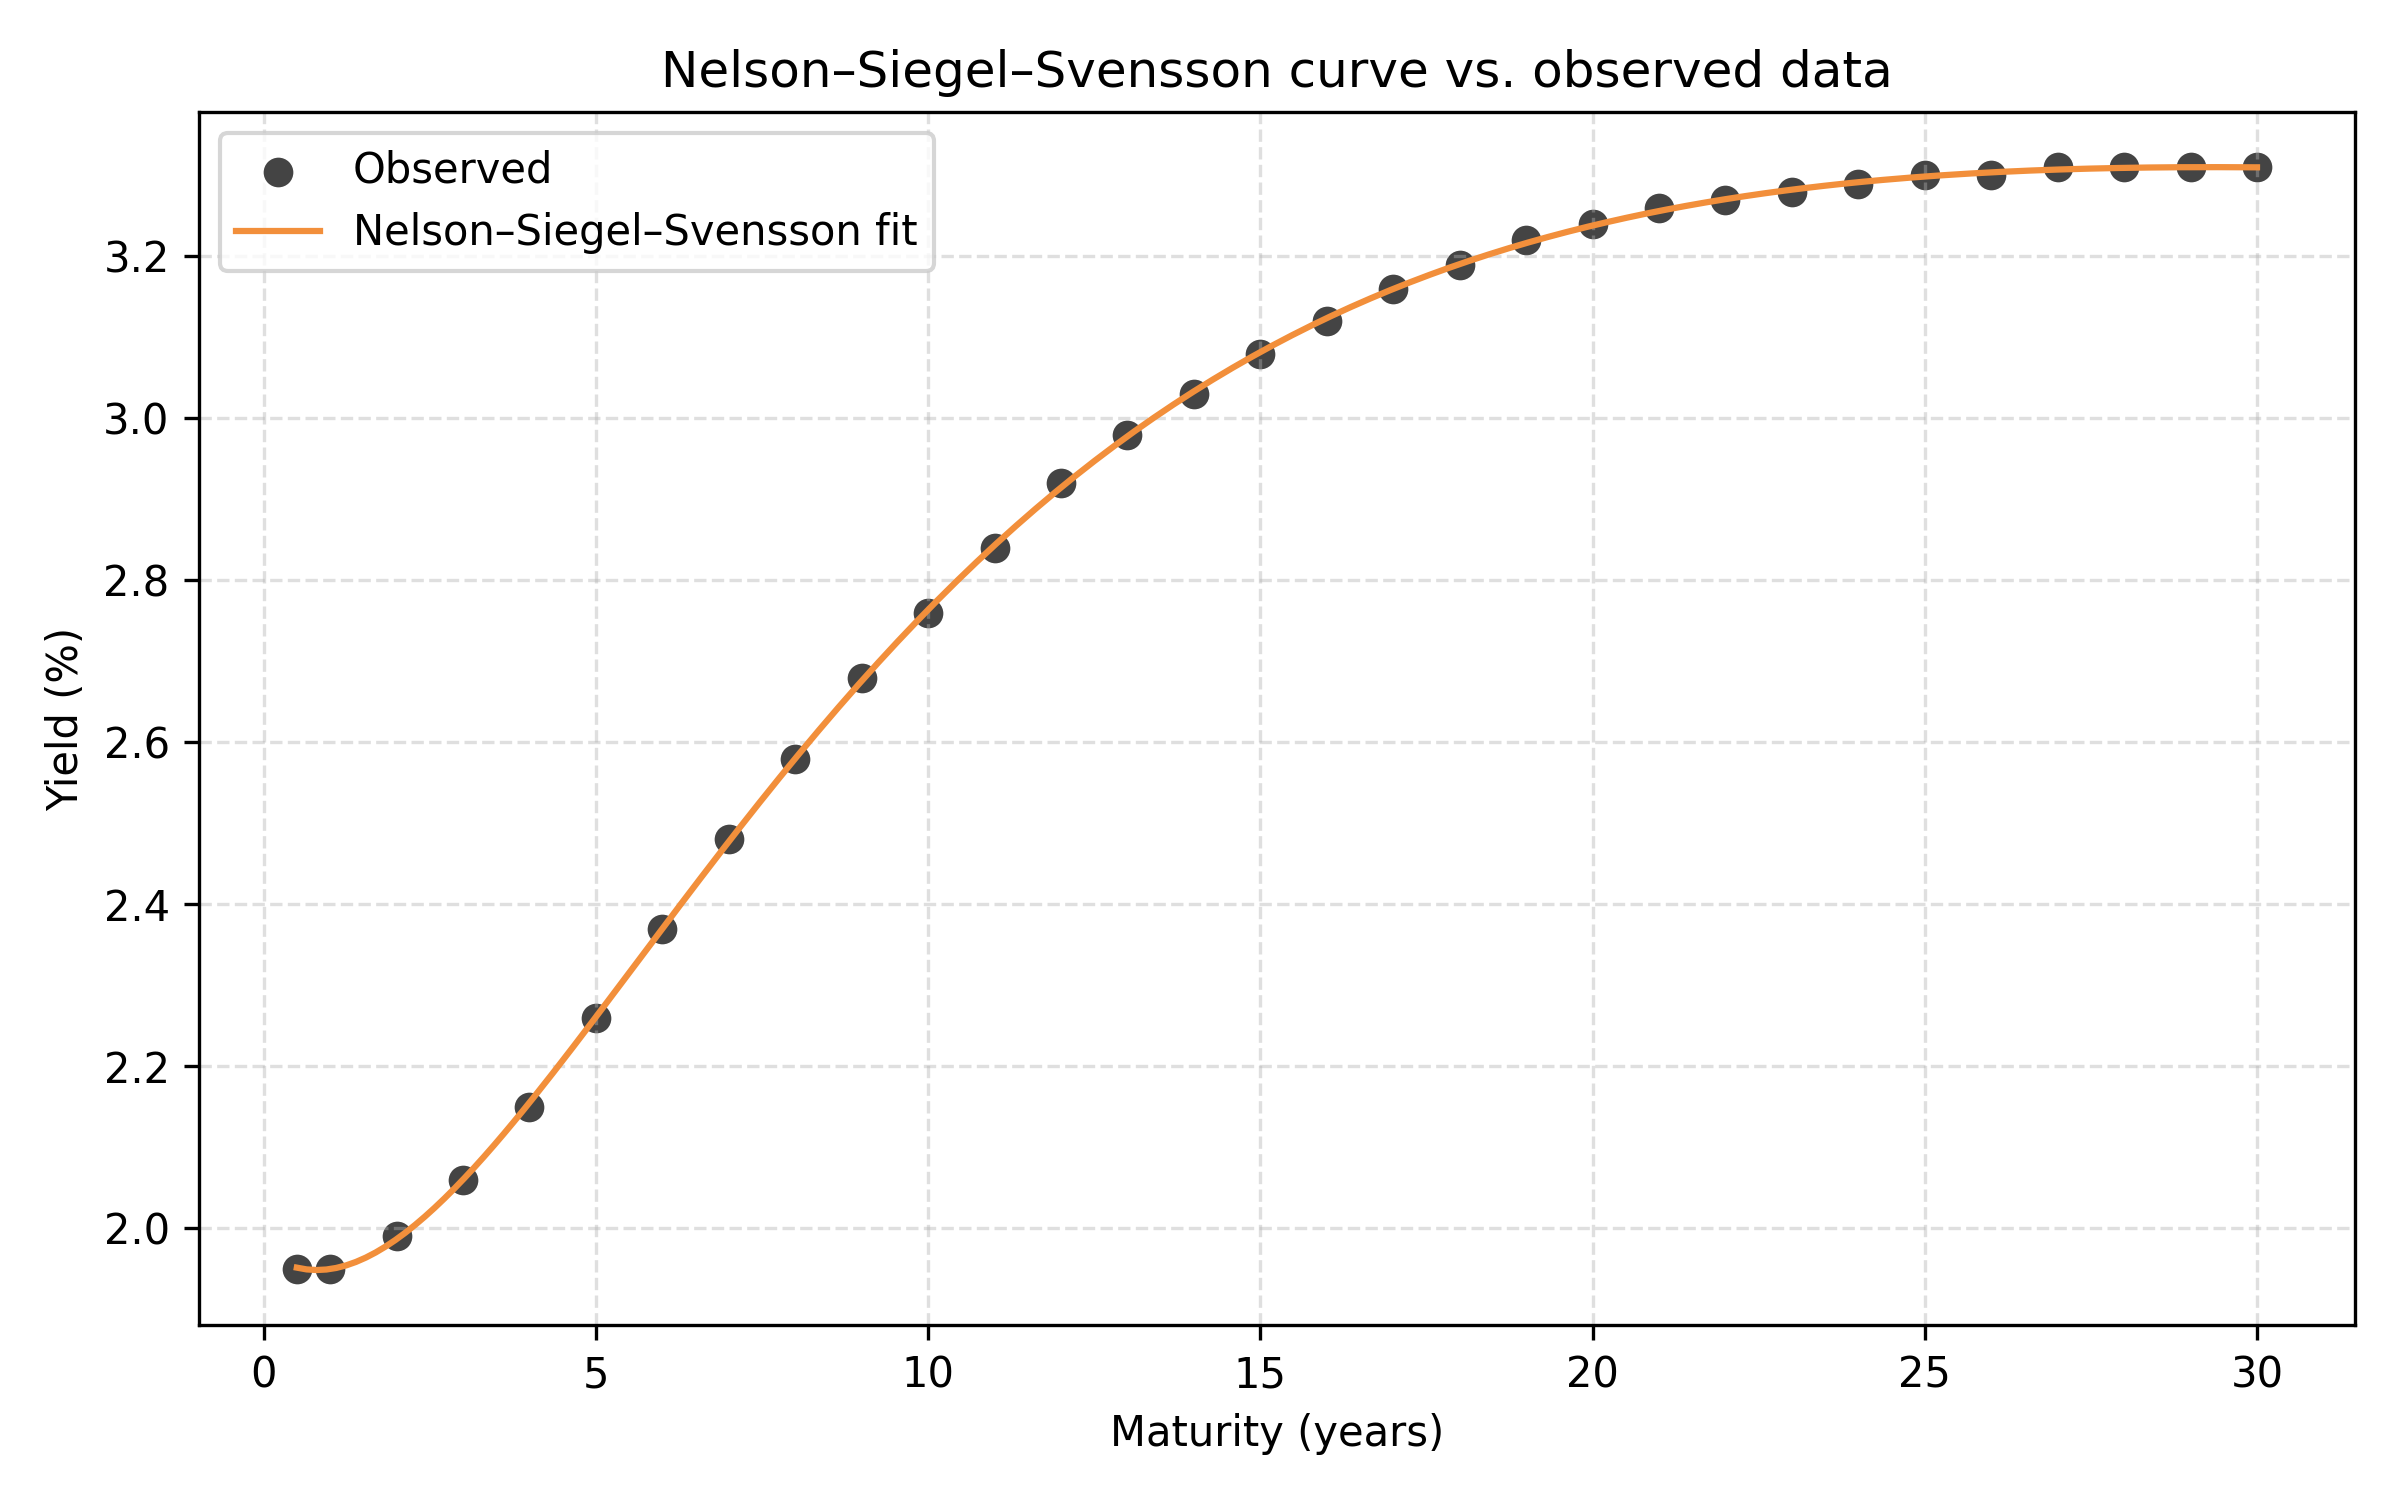
\includegraphics[width=0.8\textwidth]{../data/output/figure_nss_fit.png}
  \caption{Nelson--Siegel--Svensson fit versus observed yields.}
  \label{fig:nss-fit}
\end{figure}

\FloatBarrier
\subsection{Cubic Spline Model}
\begin{spacing}{1.15}
To benchmark a non-parametric alternative, we fit a cubic smoothing spline \parencite{cubic_spline_1989} using \inlinecode{scipy.interpolate.UnivariateSpline}. The algorithm represents the curve as a linear combination of cubic spline basis functions and determines their coefficients by minimising a weighted sum of squared errors plus a roughness penalty. We set the smoothing factor to $s = 5\times 10^{-4}$, which lets the spline nearly interpolate the 0.5--30 year observations while damping tiny wiggles that would overfit daily noise. The resulting curve is twice continuously differentiable, so forward rates implied by the first derivative remain well behaved, and the residuals stay within a few basis points across the grid.

Because the spline adapts locally, no low-dimensional parameter vector summarises its behaviour---Table~\ref{tab:param-summary} therefore lists ``--'' for the coefficient slots. Instead, interpretability hinges on diagnostics: we monitor the effective degrees of freedom (given by the number of active knots), plot the fitted curve against the raw data (Figure~\ref{fig:spline-fit}), and inspect residuals alongside the parametric models in Figure~\ref{fig:residuals}. This makes the spline a useful reference for shape, even though it cannot provide the economic narratives that Nelson--Siegel loadings offer.
\end{spacing}

\begin{figure}[htbp]
  \centering
  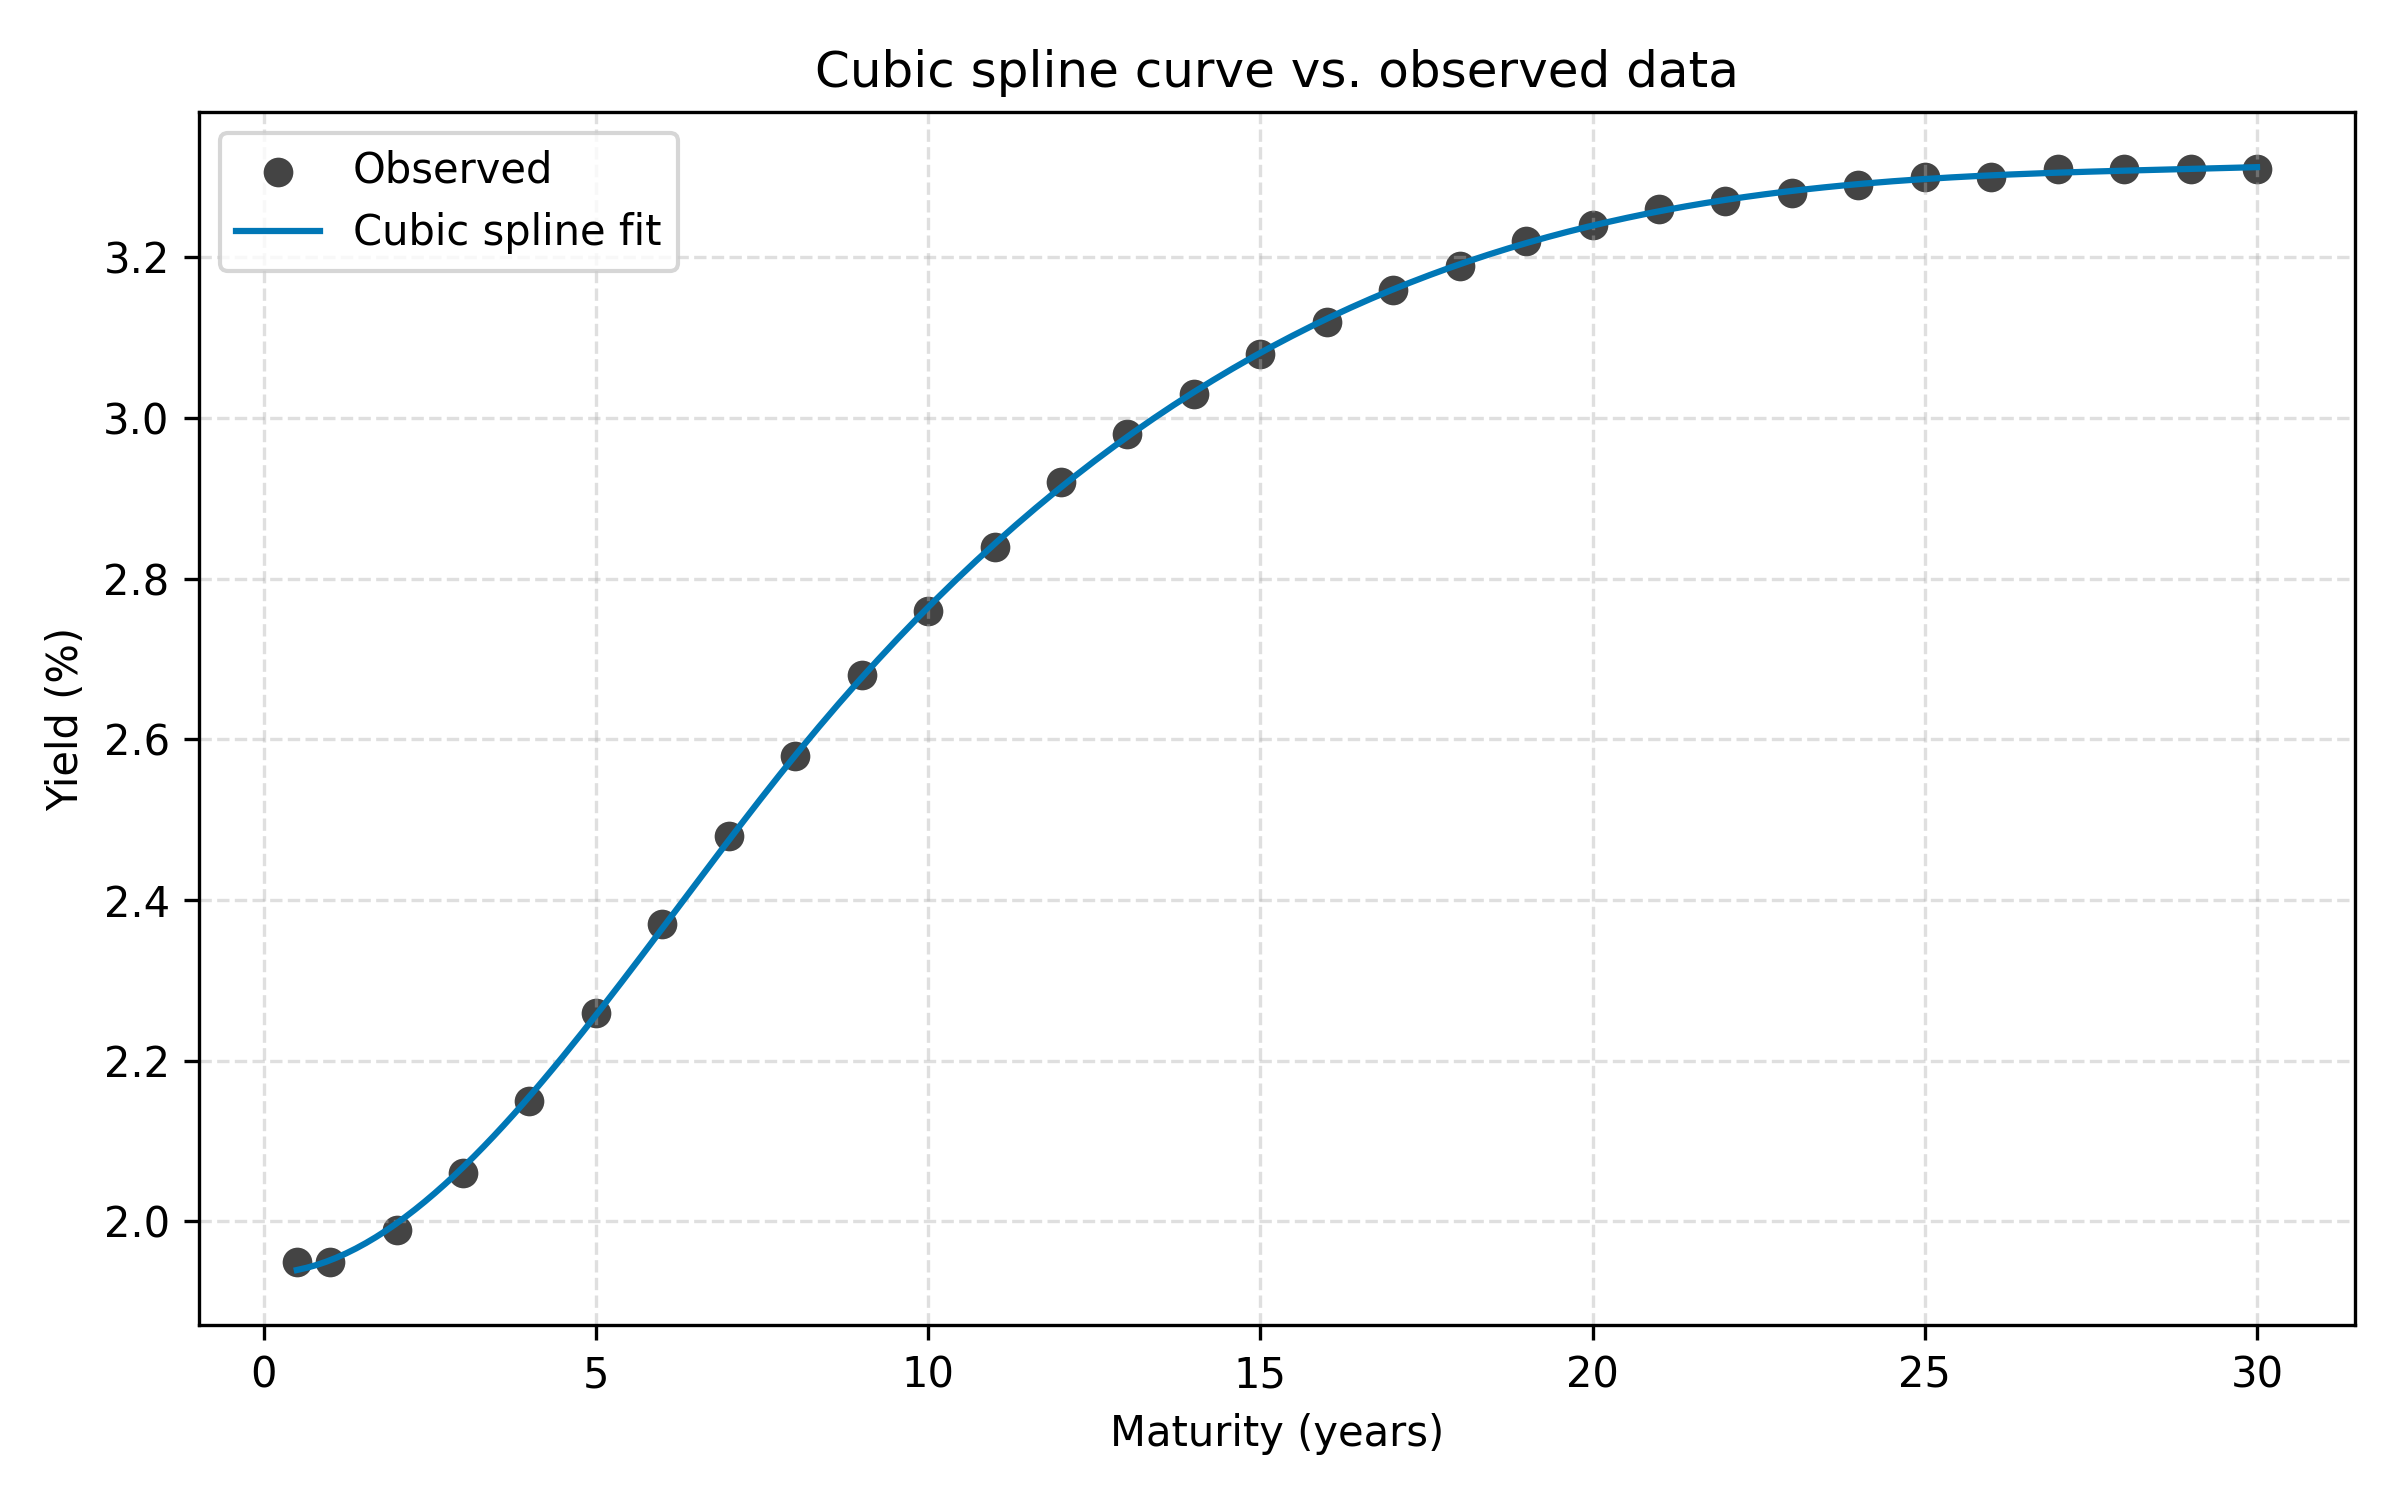
\includegraphics[width=0.8\textwidth]{../data/output/figure_spline_fit.png}
  \caption{Cubic spline fit versus observed yields.}
  \label{fig:spline-fit}
\end{figure}

\FloatBarrier
\subsection{Model Comparison and Ethics}

\begin{table}[htbp]
  \centering
  \caption{Fit diagnostics (percentage-point units).}
  \label{tab:model-metrics}
  \begin{tabular}{lrr}
\toprule
 & RMSE & MAE \\
\midrule
Nelson–Siegel & 0.0253 & 0.0222 \\
Nelson–Siegel–Svensson & 0.0027 & 0.0021 \\
Cubic spline & 0.0040 & 0.0033 \\
\bottomrule
\end{tabular}

\end{table}

\begin{table}[htbp]
  \centering
  \caption{Parameter estimates for the fitted term-structure models.}
  \label{tab:param-summary}
  \begin{tabular}{lrrrrrr}
\toprule
 & β₀ (level) & β₁ (slope) & β₂ (curvature) & β₃ (long curvature) & τ₁ (decay) & τ₂ (long decay) \\
\midrule
Nelson–Siegel & 3.6833 & -1.6349 & -2.5519 &  & 2.2657 &  \\
Nelson–Siegel–Svensson & 2.9598 & -0.9889 & -2.9529 & 3.4375 & 3.6973 & 8.3372 \\
Cubic spline &  &  &  &  &  &  \\
\bottomrule
\end{tabular}

\end{table}



\begin{spacing}{1.15}
\begin{itemize}[leftmargin=1.3em]
  \item \textbf{Fit.} Table~\ref{tab:model-metrics} shows that Nelson--Siegel--Svensson (NSS) achieves the tightest fit with an RMSE of $0.0027$ and MAE of $0.0021$, an order of magnitude smaller than the base Nelson--Siegel (NS) errors of $0.0253$ and $0.0222$. The cubic spline sits between them on accuracy (RMSE $0.0040$), closely shadowing the data yet allowing minor oscillations at very short maturities. Figure~\ref{fig:residuals} corroborates these diagnostics: NS leaves systematic underpricing at the short end and overshooting beyond 20 years, whereas NSS residuals collapse to basis-point noise across tenors and the spline residuals remain largely unbiased aside from a slight kink near the five-year node.
  \item \textbf{Interpretation.} The NS parameter set in Table~\ref{tab:param-summary} is economically intuitive but constrained. Its level factor $\beta_0=3.68\%$ anchors the long end, the slope $\beta_1=-1.63\%$ captures the downward short-to-long tilt, and the curvature $\beta_2=-2.55\%$ with decay $\tau_1=2.27$ years places the single hump around two to three years. NSS inherits that structure and adds a second pair $(\beta_3,\tau_2)=(3.44\%,8.34\text{ years})$ that bends the far end without disturbing the medium-term story, matching the observed long-end flattening. Because the spline has no finite-dimensional parameter vector (all entries are ``--'' in Table~\ref{tab:param-summary}), it offers little leverage for communicating level, slope, or curvature dynamics to stakeholders despite its solid fit.
  \item \textbf{Ethics of smoothing.} Module~2 Lesson~4 warns that concealment or distortion during smoothing can be unethical. Nelson--Siegel-type models smooth the curve, but here the process remains transparent: we report $(\beta_i,\tau_j)$ estimates, publish residual diagnostics, and retain the original Bundesbank observations. The smoothing therefore clarifies signal without hiding discrepancies, so the approach stays within ethical bounds provided the assumptions and limitations are disclosed.
\end{itemize}
\end{spacing}



\begin{figure}[htbp]
  \centering
  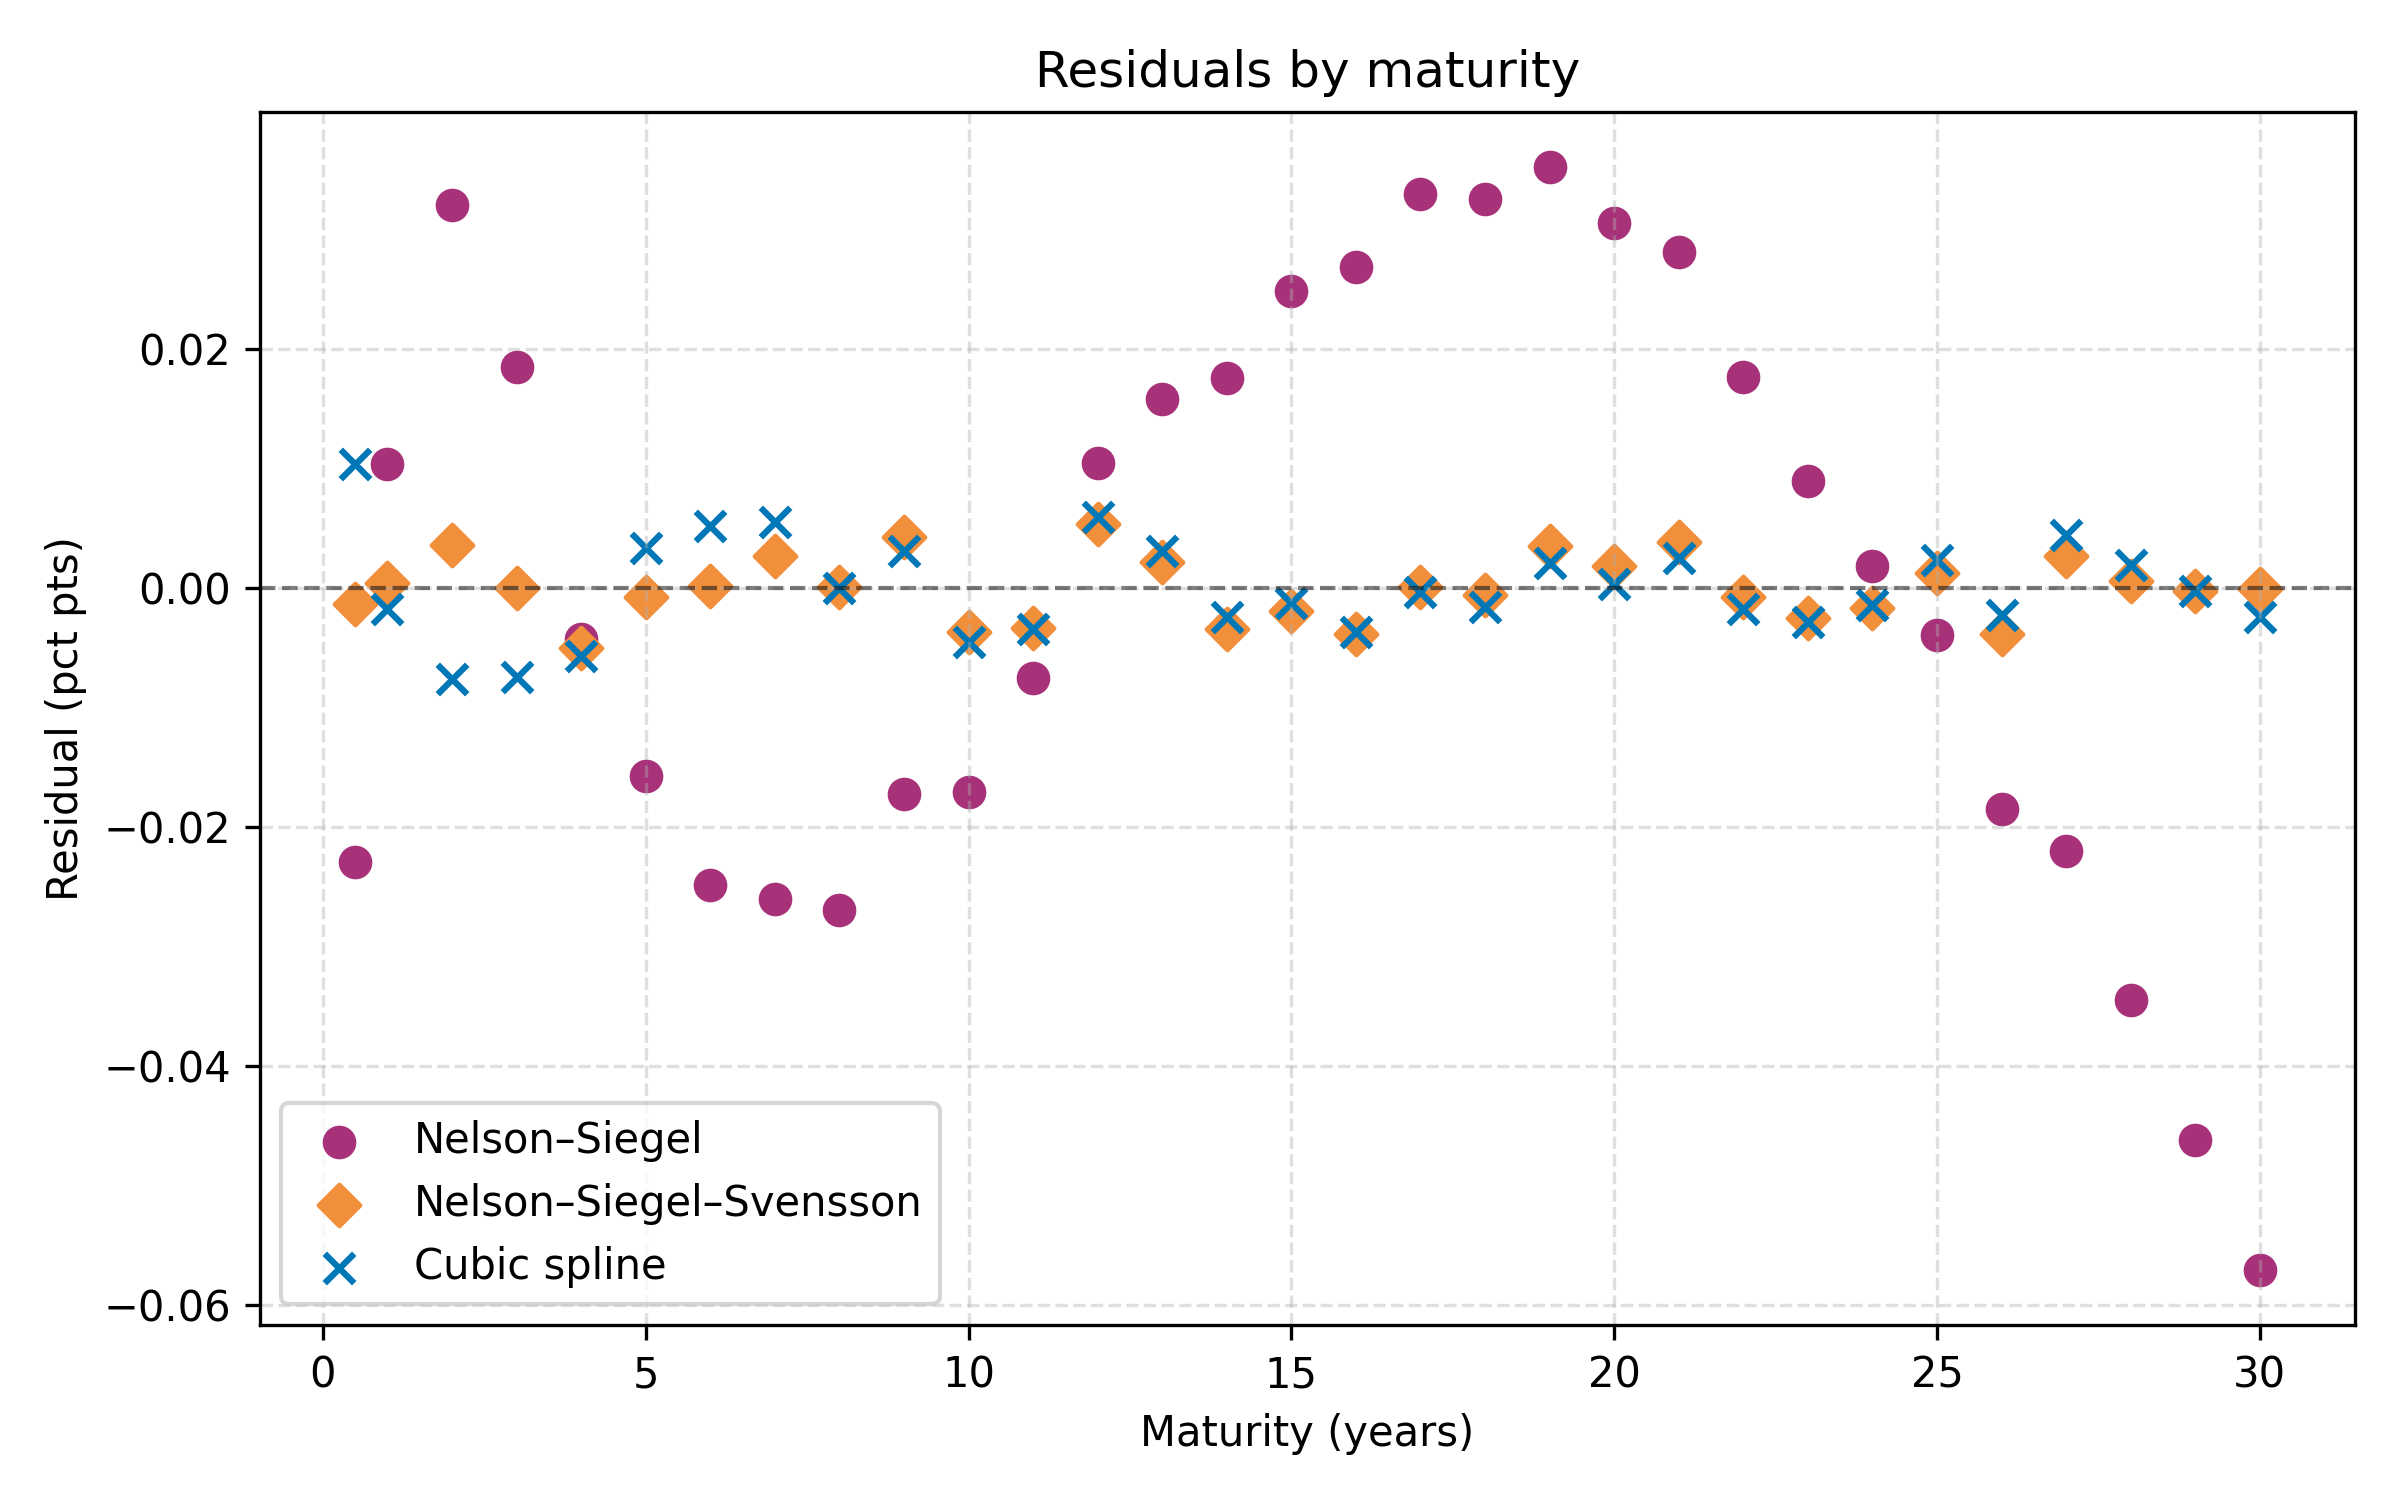
\includegraphics[width=0.8\textwidth]{../data/output/figure_model_residuals.png}
  \caption{Residuals by maturity for NS, NSS, and spline fits.}
  \label{fig:residuals}
\end{figure}

\printbibliography

\end{document}
